\documentclass[11pt,letterpaper,twoside,english]{article}

\usepackage[margin=1.4in]{geometry} % controls the size of the margins

% Special symbols, etc.
\usepackage{amssymb,amsbsy,latexsym,ytableau}
\usepackage{amsmath}
\usepackage{graphics, subfigure, float} 
\usepackage{cancel}
%\usepackage{todonotes}
% Encoding settings
\usepackage[latin1]{inputenc}
\usepackage[american]{babel}
\usepackage[T1]{fontenc} 
\usepackage{tikz}
\usepackage[scaled]{beramono}
\usepackage{listings}

\lstset{
  language=Python,
  showstringspaces=false,
  formfeed=\newpage,
  tabsize=4,
  commentstyle=\itshape,
  basicstyle=\ttfamily,
  morekeywords={while, if}
  captionpos=b,
}

\usepackage{titling} % allows posttitle command

% AMS Math packages

\usepackage{amscd,amsthm}

\usepackage{verbatim, comment} % can comment out text 
\usepackage{mdwlist} 

% Graphics
%\usepackage[dvips]{graphicx,epsfig,color}
%\usepackage{subfigure}
%\usepackage{pst-all}
%\usepackage{pstricks-add}
\usepackage{hyperref}  % can only be used with pdflatex - gives hyperlinks
\usepackage{bm} % bold math font
\usepackage{bbm}
\usepackage{pgfplots}

\renewcommand{\lstlistingname}{Algorithm}

\usepackage{todonotes}
\usepackage{caption}
\DeclareCaptionFormat{myformat}{#1#2#3\hrulefill}
\captionsetup{format=myformat}
\captionsetup[lstlisting]{position=bottom,format=myformat}

\newtheoremstyle{theorem}{1em}{1em}{\slshape}{0pt}{\bfseries}{.}{ }{}
\theoremstyle{theorem}
\newtheorem{theorem}{Theorem}[section]
\newtheorem*{theorem*}{Theorem}
\newtheorem{corollary}[theorem]{Corollary}
\newtheorem{proposition}[theorem]{Proposition}
\newtheorem{lemma}[theorem]{Lemma}
\newtheorem{claim}[theorem]{Claim}
\newtheorem{conjecture}[theorem]{Conjecture}
\newtheorem{definition}[theorem]{Definition}
\newtheorem*{claim*}{Claim}

\theoremstyle{remark}
\newtheorem{remark}[theorem]{Remark}
\newtheorem*{remark*}{Remark}
\newtheorem{algorithm}{Algorithm}
\newtheorem*{question*}{Question}
\newtheorem{question}{Question}
\newtheorem{example}[theorem]{Example}

\providecommand{\R}{\mathbb{R}}

\providecommand{\setN}{\mathbb{N}}
\providecommand{\setZ}{\mathbb{Z}}
\providecommand{\setQ}{\mathbb{Q}}
\providecommand{\setR}{\mathbb{R}}
\providecommand{\E}{\mathrm{E}}
\providecommand{\Pr}{\mathrm{Pr}}
\providecommand{\Var}{\mathrm{Var}}

\tikzset
{
    treenode/.style = {circle, draw=black, align=center, minimum size=1cm},
}

\makeatother

\title{Almost orthogonal vectors} 

\author{Yajit Jain, Deepak Narayanan, Leon Zhang}

\begin{document}

\maketitle

\section{Introduction}
Consider a collection of $N$ unit vectors $v_1, \ldots, v_N$ in $\mathbb R^n$. Define $\epsilon$ as
\[\epsilon=\max_{i\neq j}|v_i\cdot v_j|^2.\]
What is the minimal attainable $\epsilon$?

For $n=N$, it is clear that the optimal value of $\epsilon$ is zero, obtained by letting $v_1,\ldots, v_N$ be any orthonormal basis. And for $N>n$, we must have $\epsilon>0$ as any collection of $N$ vectors is linearly dependent, while any collection of orthonormal vectors is linearly independent. 

For fixed $n$, it is also easy to see that the minimum value of $\epsilon$ is nondecreasing as $N$ increases: that is, if $\epsilon_1$ is the minimum value of $\epsilon$ for $N$ unit vectors in $\mathbb R^n$, and $\epsilon_2$ is the minimum value of $\epsilon$ for $N+1$ unit vectors in $\mathbb R^n$, we must have 
\[\epsilon_1\leq \epsilon_2.\] 

Otherwise, given a configuration of $N+1$ vectors in $\mathbb R^n$ with $\epsilon=\epsilon_2$, we could simply remove one vector and obtain a configuration of $N$ vectors whose $\epsilon$ would be less than or equal to $\epsilon_1$.

Along the same lines, given a configuration of $N$ vectors in $n$-space with corresponding $\epsilon$, we can obtain a collection of $N+1$ vectors in $\mathbb R^{n+1}$ with the same $\epsilon$: simply embed the first $N$ vectors in $\mathbb R^{n}$, then add any vector perpendicular to the hyperplane in which the $N$ vectors lie. Hence the minimum $\epsilon$ for collections of $N+1$ vectors in $\mathbb R^{n+1}$ is upper-bounded by the corresponding $\epsilon$ for $N$ vectors in $\mathbb R^n$.

In Section 2, we shall see that for $n=2$, the minimum value of $\epsilon$ is given by 
\[\epsilon=\cos^2\pi/N.\] 

We will then derive in Section 3 a lower bound on $\epsilon$ for any choice of $n$ and $N$. In Section 4 we shall see that, for $N=n+1$, the minimum value of $\epsilon$ is given by
\[\epsilon=\frac{1}{n^2},\] 
and this configuration is produced when the $n+1$ vectors point to the vertices of the $n$-simplex. We will also exhibit an optimal configuration of six vectors in $\mathbb R^3$; this optimal configuration produces an $\epsilon$ equal to
\[\epsilon=\frac 1 5.\]

In Section 5, we present the results of a computational approach to computing minimal values of $\epsilon$. Finally, in Section 6 we consider the related problem of minimizing 
\[\delta=\max_{i\neq j}v_i\cdot v_j.\]
In particular, we will show that in the case where $N=n+1$, the simplex remains the optimal configuration.

\section{$n=2$, generic $N$}
In this section, we consider the problem of almost orthogonal vectors of dimensionality $2$.

As stated previously, when $N=2$ we can easily obtain an $\epsilon$ equal to $0$; a simple example of such a configuration is $[1, 0]^T$ and $[0, 1]^T$. 

The problem, however, gets harder for larger $N$. Let us first consider the specific case of $N=3$. Once we build some intuition for the problem, we will generalize the result for arbitrary $N$.

\begin{theorem}
For $n=2$ and $N=3$, the minimum possible $\epsilon$ is equal to $1/4$.
\end{theorem}

Before proving the above theorem, we state and prove the following lemma.

\begin{lemma}
Consider $n$ angles $\theta_1, \theta_2, \ldots, \theta_n \in [0, \pi]$ s.t. $\theta_1 + \theta_2 + \ldots + \theta_n = \pi$. Then $\alpha = \max_i \cos^2 \theta_i$ must equal $\cos^2 \theta_j$ where $j = \text{argmin }\theta_i$.
\end{lemma}

\begin{proof}

\begin{figure}[!h]
	\centering
	\begin{tikzpicture}
		\begin{axis}[%
			axis x line=center, axis y line=center,
			width=10cm,
			height=4cm,
			scale only axis,
			xmin=-5,
			xmax=5,
			xtick={1.57,  3.14, 4.71},
			xticklabels={, $\pi$, },
			extra x ticks={-4.71, -3.14, -1.57},
			extra x tick labels={, $-\pi$,},
			extra x tick style={
			    xticklabel style={yshift=0.5ex, anchor=south}
			},
			ymin=-1.4,
			ymax=1.4,
			ytick={-1,  0,  1}]]
			\addplot[domain=-2*pi:2*pi,smooth] (\x,{cos(\x r)});
		\end{axis}
	\end{tikzpicture}
	\caption{Plot of $\cos \theta$ versus $\theta$}
\end{figure}

Our argument hinges on the fact that for all $\theta \in [0, \pi/2]$, the function $\cos \theta$ is decreasing -- this is easy to see from Figure $1$.

Without loss of generality, let us assume that $\theta_1 \geq \theta_2 \geq \ldots \geq\theta_n$. Hence our theorem statement is equivalent to proving that $\alpha$ is equal to $\cos^2 \theta_n$.

We split our proof into two cases,
\begin{itemize}
\item $\theta_1, \theta_2, \ldots, \theta_n \in [0, \pi/2]$: In this case, it is easy to see that $\alpha = \cos^2 \theta_n$ from the fact that $\cos \theta$ is a decreasing function in $\theta$ if $\theta \in [0, \pi/2]$.

\item One of $\theta_1, \theta_2, \dots, \theta_n$ is greater than $\pi/2$:

Then, if $\theta_1 > \pi/2$ we see that $\cos^2 \theta_1 = \cos^2 (\pi - \theta_1)$ which is equal to $\cos^2 (\theta_2 + \theta_3 + \ldots + \theta_n)$. Furthermore, $\pi - \theta_1 = \theta_2 + \theta_3 + \ldots + \theta_n < \pi/2$, which means $\cos^2 \theta_1 = \cos^2 (\theta_2 + \theta_3 + \ldots + \theta_n) < \cos^2 \theta_n$. (since $\theta_n < \theta_2 + \theta_3 + \ldots + \theta_n$)

In addition, we see that for all $i \in \{2, 3, \ldots, n-1\}$, $\cos^2 \theta_i < \cos^2 \theta_n$, from which we can conclude that in this case too, $\alpha$ is equal to $\cos^2 \theta_n$.

\end{itemize}
\end{proof}

Given this lemma, we now prove the theorem stated above.

\begin{proof}
Observe that for $N=3$, the quantity $\epsilon$ for three unit-length vectors $v_1, v_2, v_3 \in \mathbb{R}^2$ is given by $$\max \{ |v_1 \cdot v_2|^2, |v_1 \cdot v_3|^2, |v_2 \cdot v_3|^2 \}$$

Since we don't care about the sign of the dot products between any two vectors (we're looking at the squares of the dot products in the above equation), and since $$|v \cdot v'| = |v \cdot (-v')|$$ for some arbitrary vector $v'$, we see that it's easy to transform the three vectors $v_1$, $v_2$ and $v_3$ so that they all lie in the same semi-circle -- to accomplish this, at most one vector needs to be reflected about the origin (multiplied by $-1$).

Without loss of generality, let $v_1 = [1, 0]^T$. Also, without loss of generality let us assume that $v_2$ and $v_3$ are above the $x$-axis, and that $v_1$, $v_2$ and $v_3$ are in anti-clockwise order.

\begin{figure}[!h]
    \centering
    \begin{tikzpicture}[yscale=-1] 
        % x-axis
        \draw [thick,->] (-4.5, 0) -- (4.5, 0);
        % y-axis
        \draw [thick,->] (0, 4.5) -- (0, -4.5);
        % origin label
        \node at (-0.5, 0.3) {\text{$(0, 0)$}};
        % x-axis label
        \node at (4.5, 0.5) {\text{$x$}};
        % y-axis label
        \node at (0, -5) {\text{$y$}};
        % circle
        \draw (0,0) circle (3cm);
        \draw (3,0)[blue,fill=blue] circle (0.1cm);
        \draw (1.5, -2.59)[blue,fill=blue] circle (0.1cm);
        \draw (-1.5, -2.59)[blue,fill=blue] circle (0.1cm);
        
        \draw [thick,-,blue] (3, 0) -- (0, 0);
        \draw [thick,-,blue] (1.5, -2.59) -- (0, 0);
        \draw [thick,-,blue] (-1.5, -2.59) -- (0, 0);
        
        \node at (4, -0.3) {\text{$v_1 = [1,0]$}};
        \node at (2.8, -3.1) {\text{$v_2 = [\cos \pi/3,\sin \pi/3]$}};
        \node at (-2.8, -3.1) {\text{$v_3 = [\cos 2\pi/3,\sin 2\pi/3]$}};
    \end{tikzpicture}
    \caption{A configuration of three unit vectors that produce the optimum $\epsilon$ for $n=2, N=3$}
\end{figure}


Let $\theta_1$ be the angle between $v_1$ and $v_2$ and $\theta_2$ be the angle between $v_2$ and $v_3$. Let us now define $\theta_3$ such that $\theta_1 + \theta_2 + \theta_3 = \pi$. Observe that $|v_1 \cdot v_3|^2 = \cos^2(\theta_1 + \theta_2) = \cos^2 (\pi - \theta_3) = \cos^2 \theta_3$, hence we can conclude that

$$\epsilon = \max_{i \in \{1,2,3\}} \cos ^2 \theta_i$$

From the above lemma, we can conclude that if $j = \text{argmin } \theta_i$ and $\theta_1 + \theta_2 + \theta_3 = \pi$, then $\epsilon = \cos^2 \theta_j$.

Furthermore, we can obtain an upper bound on $\theta_j$ by observing that $\theta_ 1 + \theta_ 2 + \theta_3 \geq \theta_ j + \theta_j + \theta_j = 3 \theta_j \Rightarrow \theta_j \leq \pi/3$. Since we're interested in the smallest such $\epsilon$ and since the cosine function is a decreasing function in $\theta$ between $0$ and $\pi/2$, we conclude that the optimum value of $\epsilon$ for $n=2$ and $N=3$ is $\cos^2 \pi / 3$. Figure $2$ shows this optimum configuration.

\end{proof}

Given the above result for $N=3$, we attempt to generalize to any integer $N$ in the following theorem.

\begin{theorem}
For $n=2$ and arbitrary $N$, the optimum value of $\epsilon$ is given by $\cos^2 \pi/N$.
\end{theorem}

\begin{proof}
The proof of this theorem is similar to the proof for the specific case of $N=3$.

Again without loss of generality, we can assume that the vectors $v_1, v_2, \ldots, v_N$ are on or above the $x$-axis, and that $v_1 = [1,0]^T$ -- if any vector $v_i$ were not above the $x$-axis, then we could just consider $-v_i$ (the reflection of $v_i$ about the $x$-axis) instead.

Let us define $\theta_i$ as the angle between the vectors $v_i$ and $v_{i+1}$ for $i \in \{1, 2, \ldots, N-1\}$, and let $\theta_N$ be the angle such that $\theta_1 + \theta_2 + \ldots + \theta_N = \pi$.

Observe that as before, we are interested in maximizing the square of the cosine of the angle between any two vectors in $v_1, v_2, \ldots, v_N$. Note that here, the angle between any two vectors in $v_j$ and $v_k$ in $v_1, v_2, \ldots, v_N$ can be expressed as $\sum_{i=j} ^{k-1} \theta_i$. Note that, however, if $\sum_{i=j}^{k-1} \theta_i \leq \pi/2$, then $\cos^2 \theta_j \geq \cos^2(\sum_{i=j}^{k-1} \theta_i)$ and that if $\sum_{i=j}^{k-1} \theta_i > \pi/2$, then $\cos^2 (\sum_{i=j}^{k-1} \theta_i) = \cos^2 (\pi - \sum_{i=j}^{k-1} \theta_i)$ which is less than $\cos^2 \theta_i$ for any $i$ in $$\{1, 2, \ldots, N-1, N\} \setminus \{j, j+1, \ldots, k-1\}$$, where $j, k \in \{1, 2, \ldots, N-1\}$ and $j \neq k$.

From this we can conclude that $\epsilon$ is equal to $\max_i \cos^2 \theta_i$. Then, if $j = \text{argmin } \theta_i$, then we see that $\epsilon = \cos^2 \theta_j$ by Lemma $2.2$.

Since $\theta_ 1 + \theta_2 + \ldots + \theta_N \geq N \cdot \theta_j \Rightarrow \theta_j \leq \pi/N$, we conclude that the optimum $\epsilon$ value is in fact equal to $\cos^2 \pi/N$ (again making use of the fact that the cosine function is decreasing between $0$ and $\pi/2$).
\end{proof}

\begin{figure}[!h]
    \centering
    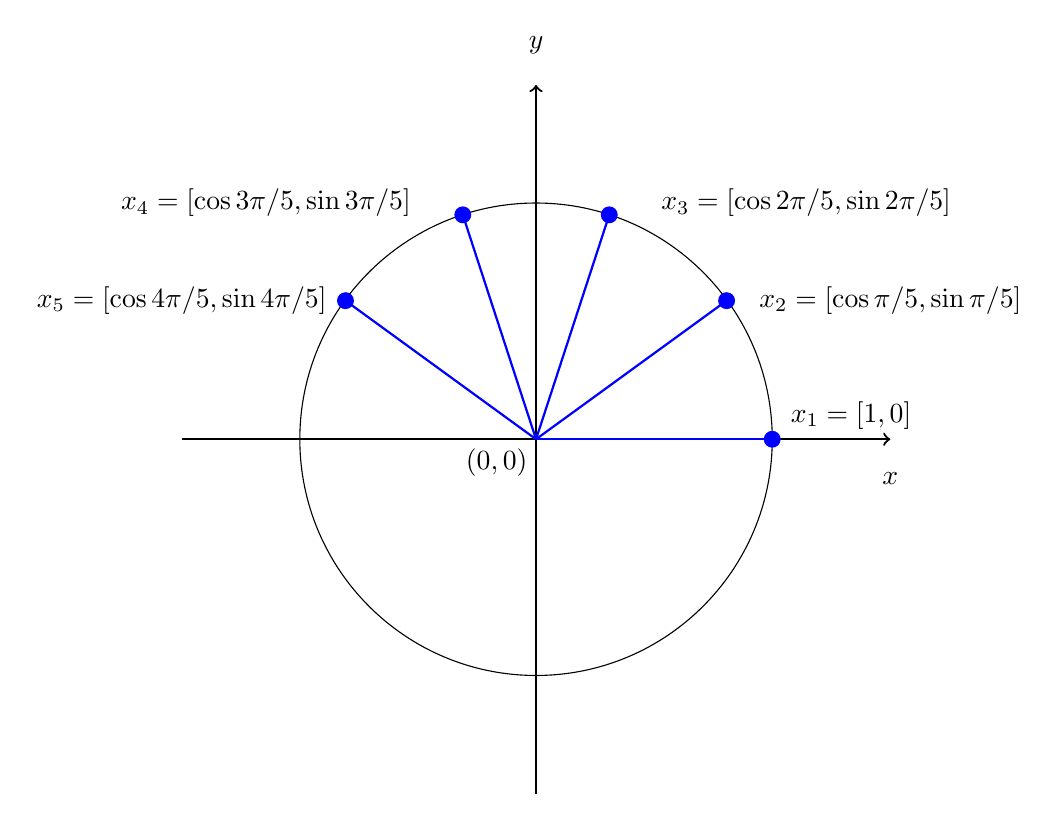
\begin{tikzpicture}[yscale=-1] 
        % x-axis
        \draw [thick,->] (-4.5, 0) -- (4.5, 0);
        % y-axis
        \draw [thick,->] (0, 4.5) -- (0, -4.5);
        % origin label
        \node at (-0.5, 0.3) {\text{$(0, 0)$}};
        % x-axis label
        \node at (4.5, 0.5) {\text{$x$}};
        % y-axis label
        \node at (0, -5) {\text{$y$}};
        % circle
        \draw (0,0) circle (3cm);
        \draw (3,0)[blue,fill=blue] circle (0.1cm);
        \draw (2.42, -1.76)[blue,fill=blue] circle (0.1cm);
        \draw (0.93, -2.85)[blue,fill=blue] circle (0.1cm);
        \draw (-2.42, -1.76)[blue,fill=blue] circle (0.1cm);
        \draw (-0.93, -2.85)[blue,fill=blue] circle (0.1cm);
        
        \draw [thick,-,blue] (3, 0) -- (0, 0);
        \draw [thick,-,blue] (2.42, -1.76) -- (0, 0);
        \draw [thick,-,blue] (0.93, -2.85) -- (0, 0);
        \draw [thick,-,blue] (-2.42, -1.76) -- (0, 0);
        \draw [thick,-,blue] (-0.93, -2.85) -- (0, 0);
        
        \node at (4, -0.3) {\text{$x_1 = [1,0]$}};
        \node at (4.5, -1.76) {\text{$x_2 = [\cos \pi/5,\sin \pi/5]$}};
        \node at (3.43, -3) {\text{$x_3 = [\cos 2\pi/5,\sin 2\pi/5]$}};
         \node at (-4.5, -1.76) {\text{$x_5 = [\cos 4\pi/5,\sin 4\pi/5]$}};
        \node at (-3.43, -3) {\text{$x_4 = [\cos 3\pi/5,\sin 3\pi/5]$}};
    \end{tikzpicture}
    \caption{A configuration of five unit vectors that produce the optimum $\epsilon$ for $n=2, N=5$}
\end{figure}

\begin{figure}[!h]
    \centering
    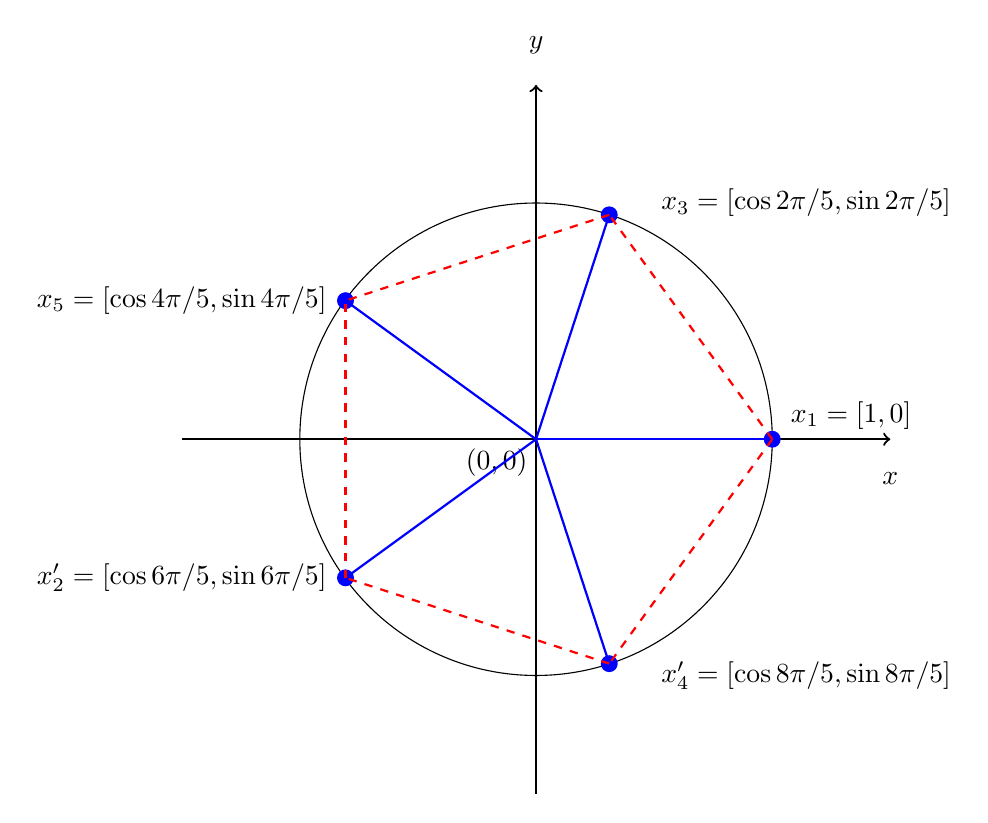
\begin{tikzpicture}[yscale=-1] 
        % x-axis
        \draw [thick,->] (-4.5, 0) -- (4.5, 0);
        % y-axis
        \draw [thick,->] (0, 4.5) -- (0, -4.5);
        % origin label
        \node at (-0.5, 0.3) {\text{$(0, 0)$}};
        % x-axis label
        \node at (4.5, 0.5) {\text{$x$}};
        % y-axis label
        \node at (0, -5) {\text{$y$}};
        % circle
        \draw (0,0) circle (3cm);
        \draw (3,0)[blue,fill=blue] circle (0.1cm);
        \draw (-2.42, 1.76)[blue,fill=blue] circle (0.1cm);
        \draw (0.93, -2.85)[blue,fill=blue] circle (0.1cm);
        \draw (-2.42, -1.76)[blue,fill=blue] circle (0.1cm);
        \draw (0.93, 2.85)[blue,fill=blue] circle (0.1cm);
        
        \draw [thick,-,blue] (3, 0) -- (0, 0);
        \draw [thick,-,blue] (-2.42, 1.76) -- (0, 0);
        \draw [thick,-,blue] (0.93, -2.85) -- (0, 0);
        \draw [thick,-,blue] (-2.42, -1.76) -- (0, 0);
        \draw [thick,-,blue] (0.93, 2.85) -- (0, 0);
        
        \node at (4, -0.3) {\text{$x_1 = [1,0]$}};
        \node at (-4.5, 1.76) {\text{$x'_2 = [\cos 6\pi/5,\sin 6\pi/5]$}};
        \node at (3.43, -3) {\text{$x_3 = [\cos 2\pi/5,\sin 2\pi/5]$}};
         \node at (-4.5, -1.76) {\text{$x_5 = [\cos 4\pi/5,\sin 4\pi/5]$}};
        \node at (3.43, 3) {\text{$x'_4 = [\cos 8\pi/5,\sin 8\pi/5]$}};
        
        \draw [thick,-,red,dashed] (3, 0) -- (0.93, 2.85);
        \draw [thick,-,red,dashed] (3, 0) -- (0.93, -2.85);
        \draw [thick,-,red,dashed] (0.93, 2.85) -- (-2.42, 1.76);
        \draw [thick,-,red,dashed] (0.93, -2.85) -- (-2.42, -1.76);
        \draw [thick,-,red,dashed] (-2.42, 1.76) -- (-2.42, -1.76);
    \end{tikzpicture}
    \caption{A configuration of five unit vectors that produce the optimum $\epsilon$ for $n=2, N=5$ with $x_2$ and $x_4$ from the previous figure reversed}
\end{figure}

Figure $3$ shows an optimum configuration for $n=2$ and $N=5$. Note by taking reflections of $x_2$ and $x_4$ in Figure $3$, we get five vectors that form a regular $5$-gon -- this can be seen in Figure $4$. A similar transformation can be done for all odd $N$.

\section{A lower bound}

In the search for a lower bound on $\epsilon$ for arbitrary $(n, N)$ pairs, it is natural to consider the so-called \emph{Gram matrix} of our collection of vectors. 
\begin{definition}
The Gram matrix of a collection of $N$ vectors $v_1,\ldots, v_N$ in $\mathbb R^n$ is the $N$-by-$N$ matrix given by
\[G(v_1,\ldots, v_N)=\left(\begin{matrix}
v_1\cdot v_1 & v_1\cdot v_2 & \ldots & v_1\cdot v_n\\
v_2\cdot v_2 & v_2\cdot v_2 & \ldots & v_2\cdot v_n\\
\vdots & \vdots & \ddots & \vdots\\
v_n\cdot v_1 & v_n\cdot v_2 & \ldots & v_n\cdot v_n\end{matrix}\right).\]
\end{definition}
Note that the Gram matrix can be written as the product $A^TA$, where $A$ is the $n$-by-$N$ matrix
\[A=\left(\begin{matrix}
| & | & \cdots & | & |\\
v_1 & v_2 & \cdots & v_{N-1} & v_N\\
| & | & \cdots & | & | \end{matrix}\right).\]
We can use a well-known lemma on the rank of certain real symmetric matrices to derive a useful lower bound. Our proof of the lemma follows that of a paper by Noga Alon\footnote{Lemma 2.2, \emph{Perturbed identity matrices have high rank: proof and applications}, Noga Alon.}.

\begin{lemma}
Let $A=(a_{i,j})$ be an $n$-by-$n$ real symmetric matrix with $a_{i,i}=1$ for all $i$ and $|a_{i,j}|\leq \sqrt{\epsilon}$ for all $i\neq j$. Let $d$ be the rank of $A$. Then
\[\epsilon\geq \frac{n-d}{d(n-1)}.\]
\end{lemma}
\begin{proof}
We define $\lambda_1,\ldots, \lambda_n$ to be the eigenvalues of $A$; write $k$ as the number of nonzero eigenvalues. Their sum is the trace of $A$, equal to $n$. We know that the number of nonzero eigenvalues of a complex matrix is less than or equal to the rank of the matrix: so we have that $d\geq k$.

Recall the Cauchy-Schwarz for $\mathbb R^n$: given $(x_1,\ldots, x_n)$ and $(y_1,\ldots, y_n)\in \mathbb R^n$, we have
\[\left(\sum_{i=1}^nx_iy_i\right)^2\leq \left(\sum_{i=1}^n x_i^2\right)\left(\sum_{i=1}^ny_i^2\right).\]
In our case, let the $x_i$ equal $\lambda_i$, and let each $y_i$ equal 1 when $\lambda_i$ is nonzero and zero when $\lambda_i$ is zero. We get
\[n^2=\left(\sum_{i=1}^n \lambda_i\right)^2\leq \left(\sum_{i=1}^n \lambda_i^2\right) k\]
so that
\[\sum_{i=1}^n \lambda_i^2\geq\frac{n^2}{k}\geq \frac{n^2}{d}.\]
In fact, the sum $\sum_{i=1}^n \lambda_i^2$ is equal to the trace of $A^TA$, which we can compute explicitly to be $\sum_{i,j}a_{i,j}^2$. Hence we have that
\[\sum_{i,j}a_{i,j}^2\geq \frac{n^2}{d}.\]
But because $|a_{i,j}|\leq \sqrt\epsilon$ for $i\neq j$, we can bound the left hand side:
\[n+n(n-1)\epsilon\geq \left(\sum_{i=1}^j a_{i,i}^2\right)+\left(\sum_{i\neq j}a_{i,j}^2\right)=\sum_{i,j}a_{i,j}^2.\]
We obtain, therefore, that
\[n+n(n-1)\epsilon\geq \frac{n^2}{d},\]
and it clearly follows that
\[\epsilon\geq \frac{n-d}{d(n-1)}.\]
\end{proof}
Using this lemma, we can now prove our lower bound on $\epsilon$.
\begin{theorem}
\label{lower_bound}
For any choice of $n$ and $N$, the minimum value of $\epsilon$ satisfies
\[\epsilon\geq \frac{N-n}{n(N-1)}.\]
\end{theorem}
\begin{proof}
Pick any collection of $N$ unit vectors $v_1,\ldots, v_N$ in $\mathbb R^n$, and define $\epsilon$ as usual. Recall the definitions of $A$ and $G$:
\[A=\left(\begin{matrix}
| & | & \cdots & | & |\\
v_1 & v_2 & \cdots & v_{N-1} & v_N\\
| & | & \cdots & | & | \end{matrix}\right).\] 
\[G(v_1,\ldots, v_N)=A^TA=\left(\begin{matrix}
v_1\cdot v_1 & v_1\cdot v_2 & \ldots & v_1\cdot v_n\\
v_2\cdot v_2 & v_2\cdot v_2 & \ldots & v_2\cdot v_n\\
\vdots & \vdots & \ddots & \vdots\\
v_n\cdot v_1 & v_n\cdot v_2 & \ldots & v_n\cdot v_n\end{matrix}\right).\]
Let $d$ be the rank of $G$. Since $A$ has rank at most $n$, so does $A^T$; since the image space of $G$ must be contained in the image space of $A^T$, we must have that $d\leq n$. Note that $G$ is real and symmetric, with $1$s along the diagonal and all other entries with absolute value bounded by $\sqrt \epsilon$. We can apply the lemma to conclude
\[\epsilon\geq \frac{N-d}{d(N-1)}.\]
Since $d\leq n$, we have as desired
\[\epsilon\geq \frac{N-n}{n(N-1)}.\]
\end{proof}
We present now a table of the bounds the theorem gives to us for varying $n$ and $N$:
\begin{table}[h]
   \centering
    \begin{tabular}{ | c | c | c | c |}
    \hline
      & $n=2$ & $n=3$ & $n=4$ \\ \hline
    $N=2$ & $0$ & $-$ & $-$ \\ \hline
    $N=3$ & $1/4$ & $0$ & $-$ \\ \hline
    $N=4$ & $1/3$ & $1/9$ & $0$ \\ \hline
    $N=5$ & $3/8$ & $1/6$ & $1/16$ \\ \hline
    $N=6$ & $2/5$ & $1/5$ & $1/10$ \\ \hline
    $N=8$ &  $3/7$ & $5/21$ & $1/7$ \\ \hline
    $N=12$ & $5/11$ & $3/11$ & $2/11$ \\
    \hline
    \end{tabular}
    \caption {Lower bounds on $\epsilon$ for different values of $(n, N)$, given by Theorem \ref{lower_bound}.}
    \end{table}

Note that the bounds for $n=2$ are not tight, as we proved in Section 2 that the minimum $\epsilon$ was given by $\cos^2(\pi/N)$. We shall see, however, that the bounds for $\epsilon$ are in fact tight in the cases where $N=n+1$ and where $n=3, N=6$. One direction for further research might be checking whether the bounds provided by Theorem \ref{lower_bound} are indeed attainable for other combinations of $n$ and $N$.

\section{Some Optimal Configurations}
Below we provide choices of $n$ and $N$ for which we can achieve the lower bound given by Theorem ~\ref{lower_bound}.
\subsection{$n=3,N=6$}
In this situation we have a lower bound of $\epsilon\ge\frac{1}{5}$ from the above theorem. Consider the following 6 vectors on the unit sphere in $\R^3$ with variables $a$ and $b$. 
$$
(a,b,0),(a,0,b),(b,0,a)
$$
$$
(a,-b,0),(a,0,-b),(-b,0,a)
$$
There are three possible dot products we get from computing dot products between non-equal vectors chosen from these six vectors: $ab,-ab,a^2-b^2$. This gives us two possible values of $\epsilon$: $(a^2-b^2)^2,(ab)^2$. It would seem that an optimal configuration can be obtained by setting $a^2-b^2=ab$. If we add in the constraint that $a^2+b^2=1$ (since the six vectors we're interested in must live on the unit sphere), we get
$$
a=\sqrt{\frac{1}{10}(5-\sqrt{5}}, b=-\frac{1+\sqrt{5}}{2}\sqrt{\frac{1}{10}(5-\sqrt{5}}. 
$$
If we compute $\epsilon=(a^2-b^2)^2=(ab)^2$, we see that $\epsilon=\frac{1}{5}$; coupling this knowledge with the fact that for $(n, N) = (3, 6)$, we see that these six points give us an optimal configuration.
\subsection{$N=n+1$}
Let us now consider the situation in which we try to minimize $\epsilon$ for $n+1$ vectors in an $n$ dimensional space. From Theorem ~\ref{lower_bound} we know that $\epsilon\ge \frac{1}{n^2}$, so if we show that there exist some $n+1$ vectors in $n$-space that achieve an $\epsilon$ equal to $1/n^2$, then we can conclude that $1/n^2$ is the optimal value of $\epsilon$ for $N = n+1$.

To do this, we first define what we mean by an $n$-dimensional simplex. 

\begin{definition}
An $n$-dimensional simplex is given by the convex hull of the $n+1$ points in $\R^{n+1}$ described as having a 1 in a single coordinate and zeros in every other coordinate. 
\end{definition}

Figure $5$ shows diagrams of a 2-dimensional simplex.

\begin{figure}[!h]
    \centering
        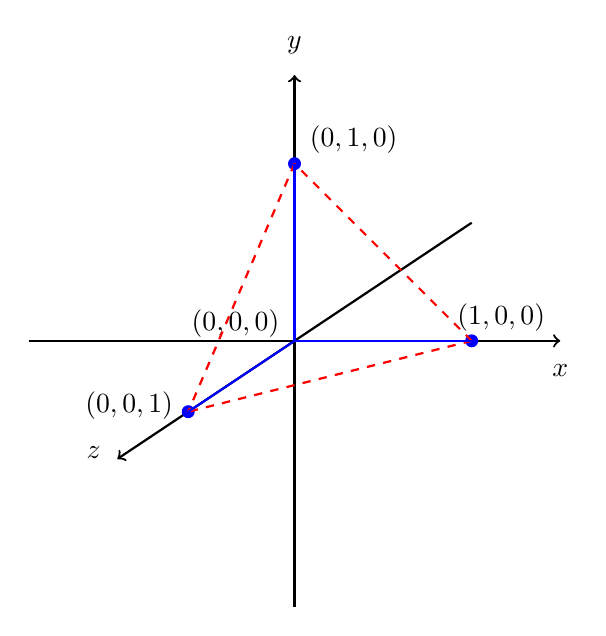
\begin{tikzpicture}[yscale=-1, scale=0.75]
        % x-axis
        \draw [thick,->] (-4.5, 0) -- (4.5, 0);
        % y-axis
        \draw [thick,->] (0, 4.5) -- (0, -4.5);
        % z-axis
        \draw [thick, ->] (3.0, -2.0) -- (-3.0, 2.0);
        % origin label
        \node at (-1, -0.3) {\text{$(0, 0, 0)$}};
        % x-axis label
        \node at (4.5, 0.5) {\text{$x$}};
        % y-axis label
        \node at (0, -5) {\text{$y$}};
         % z-axis label
        \node at (-3.4, 1.9) {\text{$z$}};
        \node at (3.5, -0.4) {\text{$(1, 0, 0)$}};
        \node at (1, -3.4) {\text{$(0, 1, 0)$}};
        \node at (-2.8, 1.1) {\text{$(0, 0, 1)$}};
        % circle
        \draw (3,0)[blue,fill=blue] circle (0.1cm);
        \draw (0, -3)[blue,fill=blue] circle (0.1cm);
        \draw (-1.8, 1.2)[blue,fill=blue] circle (0.1cm);
        
        \draw [thick,-,red,dashed] (3, 0) -- (0, -3);
        \draw [thick,-,red,dashed] (0, -3) -- (-1.8, 1.2);
        \draw [thick,-,red,dashed] (3, 0) -- (-1.8, 1.2);
        
        \draw [thick,-,blue] (3, 0) -- (0, 0);
        \draw [thick,-,blue] (0, -3) -- (0, 0);
        \draw [thick,-,blue] (-1.8, 1.2) -- (0, 0);
    \end{tikzpicture}
    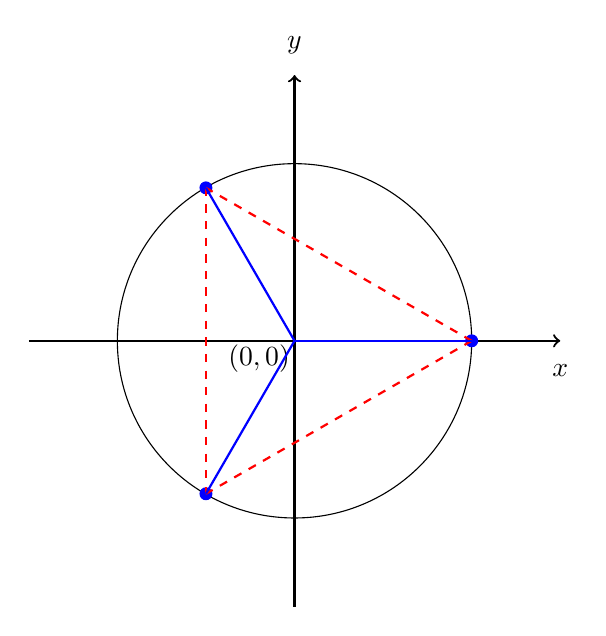
\begin{tikzpicture}[yscale=-1, scale=0.75]
        % x-axis
        \draw [thick,->] (-4.5, 0) -- (4.5, 0);
        % y-axis
        \draw [thick,->] (0, 4.5) -- (0, -4.5);
        % origin label
        \node at (-0.6, 0.3) {\text{$(0, 0)$}};
        % x-axis label
        \node at (4.5, 0.5) {\text{$x$}};
        % y-axis label
        \node at (0, -5) {\text{$y$}};
        % circle
        \draw (0,0) circle (3cm);
        \draw (3,0)[blue,fill=blue] circle (0.1cm);
        \draw (-1.5, 2.59)[blue,fill=blue] circle (0.1cm);
        \draw (-1.5, -2.59)[blue,fill=blue] circle (0.1cm);
        
        \draw [thick,-,red,dashed] (3, 0) -- (-1.5, 2.59);
        \draw [thick,-,red,dashed] (3, 0) -- (-1.5, -2.59);
        \draw [thick,-,red,dashed] (-1.5, -2.59) -- (-1.5, 2.59);
        
        \draw [thick,-,blue] (3, 0) -- (0, 0);
        \draw [thick,-,blue] (-1.5, 2.59) -- (0, 0);
        \draw [thick,-,blue] (-1.5, -2.59) -- (0, 0);
    \end{tikzpicture}

    \caption{A 2-dimensional simplex drawn in $\R^3$ on the left, and then centered at the origin in $\R^2$ on the right.}
\end{figure}

Before proceeding with the theorem, we notice that when $n=2$, the configuration of $N=3$ vectors that produced the minimum value of $\epsilon$ made up a simplex centered at the origin (an equilateral triangle). 


\begin{theorem}
If $N=n+1$ and the vectors in question are denoted $v_1,\cdots, v_N$, then over all configurations of these vectors the minimum value of $\epsilon$ for $i\neq j$ is $\frac{1}{^2n}$. This is achieved when the vectors are arranged in an $n$ dimensional simplex centered at the origin.
\label{simplex}
\end{theorem}

\begin{proof}
Let $\epsilon$ be as before for a given set of unit vectors $v_1, v_2, \ldots, v_{n+1}$. We show that the origin-centered simplex configuration of the vectors $v_1,\cdots v_{n+1}$ produces a value $\epsilon=\frac{1}{n^2}$. 

We must first describe the vectors that make up the origin centered simplex. To center our simplex at the origin we take each vector in the original simplex, and subtract from it the vector representing the centroid of the original simplex. The centroid of the original simplex takes the form $(\frac{1}{N},\frac{1}{N},\ldots,\frac{1}{N})$, so the points of the new simplex take the form
$$
\left(-\frac{1}{N},\cdots,-\frac{1}{N},\frac{N-1}{N},-\frac{1}{N},\cdots,-\frac{1}{N}\right).
$$
If we renormalize these vectors so that each vector has unit length, we get 
$$
\sqrt{\frac{N}{N-1}}\left(-\frac{1}{N},\cdots,-\frac{1}{N},\frac{N-1}{N},-\frac{1}{N},\cdots,-\frac{1}{N}\right).
$$
Now, taking the dot product between any two such vectors gives us
$$
\frac{N}{N-1}\left(-2\cdot\frac{N-1}{N^2}+(N-2)\cdot\frac{1}{N^2}\right)=\frac{N}{N-1}\cdot-\frac{1}{N}=-\frac{1}{N-1}=-\frac{1}{n}.
$$
So for this configuration $\epsilon=\frac{1}{n^2}$. By Theorem ~\ref{lower_bound} we know that $\epsilon\ge \frac{1}{n^2}$, so we have achieved the lower bound. 
\end{proof}
\section{Numerical analysis and associated conjectures}

Since visualizing in spaces of dimensionality $3$ or greater is extremely hard, we used a computational approach to compute near-optimal epsilon values for different $(n, N)$ pairs. We describe this method in greater detail below.

\begin{lstlisting}
def get_min_epsilon(n, N, num_iter, start_vectors):
    min_epsilon = 1.0  # Start off with the worst possible epsilon
    current_vectors = start_vectors
    i = 0
    while (i < num_iter):
        temperature = 1.0 / float(i + 1)

        # Get perturbing vectors
        random_vectors = get_random_vectors(n, N)

        # Now perturb current_vectors
        new_vectors = list()
        for j in xrange(N):
            new_vector = list()
            for k in xrange(n):
                new_vector.append(
                    current_vectors[j][k] + (
                    	temperature * random_vectors[j][k]))
            new_vectors.append(new_vector)
        normalize_vectors(new_vectors)
        
        # Accept change only if new_vectors produces a better epsilon
        epsilon = compute_epsilon(new_vectors)
        if epsilon < min_epsilon:
            min_epsilon = epsilon
            current_vectors = new_vectors
            i += 1

    return min_epsilon, current_vectors
\end{lstlisting}
\captionof{lstlisting}{The numerical method used to generate optimum epsilon values -- note that we call this method multiple times with different start\_vectors to obtain a reasonable epsilon estimate}

Our general intuition tells us that perturbing a set of nearly optimal vectors slightly could give us a new set of vectors that produce even a smaller epsilon value. Given this, we start off with a set of random vectors, and try to move these vectors towards smaller epsilon values.

At every iteration, we try adding a vector whose norm becomes smaller with every passing iteration, to the already computed optimal vector. We present pseudocode for this algorithm above.

Even though this approach seems simple, it actually produces remarkably precise values -- this can be verified by cross-checking with results we've already proven / conjectured in this paper, this can be seen from values in Table $2$.

In particular, the computed values for $n=2$ are pretty accurate -- the computed values for different values of $N$ are very close to the expected value of $\cos^2 \pi/N$, that we already proved in Section $2$, which makes us confident about the accuracy of this numeric method.


\begin{table}
   \centering
    \begin{tabular}{ | c | c | c | c |}
    \hline
      & $n=2$ & $n=3$ & $n=4$ \\ \hline
    $N=2$ & $0.0$ & $-$ & $-$ \\ \hline
    $N=3$ & $0.25$ & $0.0$ & $-$ \\ \hline
    $N=4$ & $0.5$ & $0.11$ & $0.0$ \\ \hline
    $N=5$ & $0.66$ & $0.21$ & $0.07$ \\ \hline
    $N=6$ & $0.75$ & $0.22$ & $0.14$ \\ \hline
    $N=7$ & $0.82$ & $0.36$ & $0.18$ \\ \hline
    $N=8$ &  $0.86$ & $0.44$ & $0.24$ \\ \hline
    $N=9$ &  $0.89$ & $0.49$ & $0.26$ \\ \hline
    $N=10$ & $0.91$ & $0.51$ & $0.32$ \\ \hline
    $N=11$ & $0.93$  & $0.55$ & $0.35$ \\ \hline
    $N=12$ & $0.94$ & $0.64$ & $0.41$ \\
    \hline
    \end{tabular}
    \caption {Minimum values of $\epsilon$ for different values of $(n, N)$, as computed by our annealing method}
\end{table}



\section{Variations}

We now consider a variation of the above problem, where we actually try to place $N$ vectors in $n$-space as far apart as possible from each other. More concretely, if we define $\delta$ as

$$\delta = \max_{i \neq j} v_i \cdot v_j$$,

then we can formalize our problem as finding the $N$ vectors $v_1, v_2, \ldots, v_N$ that minimize $\delta$.

Before proving what the optimum value of $\delta$ is for $N= n+1$, we introduce the parallelogram law.

\subsection{The Parallelogram Law}

First we give the definition of the norm on vectors in $\R^n$ in terms of the dot product:

\begin{definition}
For a vector $v\in\R^n$ the norm of $v$ is the positive value of $||v||$ given by the equation
$$
||v||^2=v\cdot v.
$$
\end{definition}
\begin{theorem}[Parallelogram Law]
For vectors $v_1,\cdots,v_n\in\R^n$, the following identity holds
$$
||v_1+\cdots+v_n||^2=\displaystyle\sum_{i=1}^n||v_i||^2+2\displaystyle\sum_{1\le i<j\le n}v_i\cdot v_j.
$$
\proof
First consider the following identity from the definition of the norm for vectors $u,v\in\R^n$:
$$
||u+v||^2=(u+v)\cdot (u+v)=u\cdot u+u\cdot v+ v\cdot u + v\cdot v=||u||^2+||v||^2+2u\cdot v.
$$
Now if we let $u=v_1$ and $v= v_2+\cdots+v_n$ we get 
$$
||v_1+v_2+\cdots+v_n||^2=||v_1||^2+||v_2+\cdots +v_n||^2+2\sum_{i=2}^n v_1\cdot v_i.
$$
If we recurse on $||v_2+\cdots +v_n||^2$ using induction we get the desired result. 
\end{theorem}


\subsection{Variations: Minimizing the dot product}
Given the above bound, we proceed to state and prove the following theorem.


\begin{theorem}
If $N=n+1$ and the vectors in question are denoted $v_1,\cdots, v_N$, then over all configurations of these vectors the minimum value of $v_i\cdot v_j$ for $i\neq j$ is $\frac{-1}{n}$. This is achieved when the vectors are arranged in an $n$ dimensional simplex centered at the origin.  
\end{theorem}

\begin{proof}
Let $\delta= \max_{i\neq j}\{v_i\cdot v_j\}$ for a given set of unit vectors $v_1, v_2, \ldots, v_{n+1}$, and let $\delta_{min}$ be the minimum possible $\delta$ obtained across all unit vectors $v_1, v_2, \ldots, v_{n+1}$. We computed in the proof of Theorem ~\ref{simplex} that for the origin centered simplex, we obtain a value of $\delta_{\min}=\frac{-1}{n}$, so $\delta_{\min}\le\frac{-1}{n}$. So we need only show that $\delta_{min} \geq -\frac{1}{n}$ as well. 


To see that $\delta_{min} \ge-\frac{1}{n}$ we use the parallelogram law.

Recall that the parallelogram law states that 

$$
||v_1+\cdots+v_{n+1}||^2=\displaystyle\sum_{i=1}^{n+1}||v_i||^2+2\displaystyle\sum_{1\le i<j\le n+1}v_i\cdot v_j.
$$
In our case we know three things. First, since the norm of any vector is greater than or equal to $0$, we can conclude that $||v_1 + \cdots + v_{n+1}||^2 \geq 0$. Second, $v_i\cdot v_j\le\delta$ for any $i<j$. Third, $||v_i||=1$. Therefore 
$$
0\le n+1+n(n+1)\delta.
$$
This implies that $\delta\ge -\frac{1}{n}$ for any set of unit vectors $v_1, v_2, \ldots, v_{n+1}$, from which we can conclude that $\delta_{min} \ge -\frac{1}{n}$ as well.

Since $\delta_{min} \le -\frac{1}{n}$ and $\delta_{min} \ge -\frac{1}{n}$, we can conclude that $\delta_{min}=-\frac{1}{n}$.
\end{proof}


\end{document}